\subsection{Complex Functions}
\subsubsection{Mapping Properties of Simple Functions}
Similar to how functions with real variables map values to a different set of values, complex functions do the same. The main difference is that with complex functions we're mapping a 2 dimensional set of inputs to a 2 dimensional set of outputs.
\[
w=f(z)=u+iv
\]
We define $z\in \mathcal{S}$ the image of $\mathcal{S}$ under $w$.\\
Some common mappings:
\begin{itemize}
    \item The identity map
    \begin{align*}
        &w=f(z)=z\\
        &\eqnsystem{u=x\\ v=y}
    \end{align*}
    \item Translation by $z_0$
    \begin{align*}
        &w=f(z)=z+z_0\\
        &\eqnsystem{u=x+x_0\\ v=y+y_0}
    \end{align*}
    \item Stretching ($a>1$) or contraction ($a<1$)
    \begin{align*}
        &w=f(z)=az=are^{i\varphi},\ a\in\R\\
        &\eqnsystem{u=ax\\ v=ay}
    \end{align*}
    \item Rotation by $\varphi_0$
    \begin{align*}
        &w=f(z)=e^{i\varphi_0}z=e^{i(\varphi+\varphi_0)}
    \end{align*}
\end{itemize}
Using these basic mapping principles we are able to lay the foundation for some more complicated mappings.\\
Ex: Find the image of $S=\brcurly{|z-1|\geq1}$ under the mapping $f(z)=\frac{1}{z}$\\
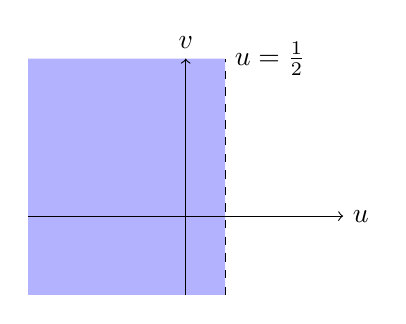
\begin{tikzpicture}
    % Region u <= 1/2
    \fill[blue!30, domain=-2:0.5, variable=\x]
        (-2, -1) -- plot ({\x}, {2}) -- (0.5, -1) -- cycle;

    % Axes
    \draw[->] (-2,0) -- (2,0) node[right] {$u$};
    \draw[->] (0,-1) -- (0,2) node[above] {$v$};
    
    % Dashed line u = 1/2
    \draw[dashed] (0.5, -1) -- (0.5, 2) node[right] {$u=\frac{1}{2}$};
\end{tikzpicture}

\begin{align*}
    &z=\frac{1}{w}=\frac{1}{u+iv}=\frac{u-iv}{u^2+v^2}\\
    &x=\frac{u}{u^2+v^2}\\
    &y=-\frac{v}{u^2+v^2}\\
    &|z-1|\geq1\Ra\brvertical{\frac{1}{w}-1}\geq1\\
    &\frac{1-w}{w}\geq1\\
    &|1-w|\geq|w|\\
    &|1-w|^2\geq|w|^2\\
    &(1-u)^2+v^2\geq u^2+v^2\\
    &-2u+1\geq 0\\
    &u\leq\frac{1}{2}\\
    &S'=\brcurly{u\leq\frac{1}{2}}
\end{align*}


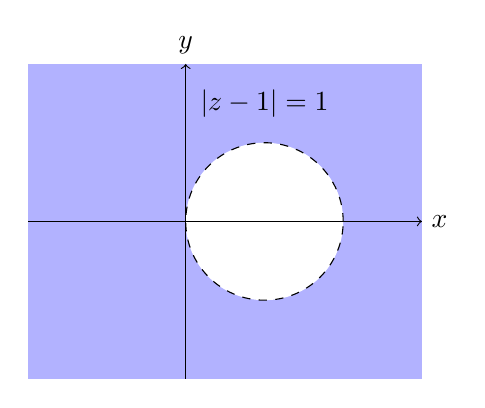
\begin{tikzpicture}
    % Background (Blue)
    \fill[blue!30] (-2,-2) rectangle (3,2);

    % Region |z-1| >= 1
    \fill[blue!30, domain=-1:1, variable=\x]
        (-2, 0) -- plot ({1+\x}, {sqrt(1 - \x*\x)}) -- (2, 0) -- cycle;
    \fill[blue!30, domain=-1:1, variable=\x]
        (-2, 0) -- plot ({1+\x}, {-sqrt(1 - \x*\x)}) -- (2, 0) -- cycle;

    % Circle (White, Dashed)
    \draw[fill=white, dashed] (1, 0) circle (1);

    % Label: |z-1| = 1
    \node at (1, 1.5) {$|z-1|=1$};

    % Axes
    \draw[->] (-2,0) -- (3,0) node[right] {$x$};
    \draw[->] (0,-2) -- (0,2) node[above] {$y$};
\end{tikzpicture}

Ex2: Find the image of $S=\brcurly{x\leq1}$ under the mapping $f(z)=\frac{1}{z}$

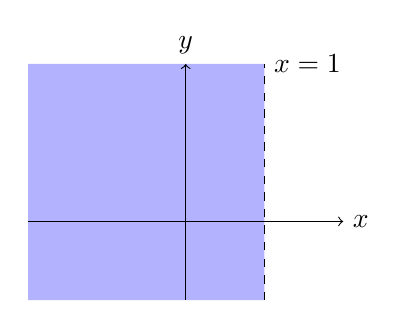
\begin{tikzpicture}
    % Region x <= 1
    \fill[blue!30, domain=-2:1, variable=\x]
        (-2, -1) -- plot ({\x}, {2}) -- (1, -1) -- cycle;

    % Axes
    \draw[->] (-2,0) -- (2,0) node[right] {$x$};
    \draw[->] (0,-1) -- (0,2) node[above] {$y$};
    
    % Dashed line x = 1
    \draw[dashed] (1, -1) -- (1, 2) node[right] {$x=1$};
\end{tikzpicture}
\begin{align*}
    &z=\frac{1}{w}=\frac{1}{u+iv}=\frac{u-iv}{u^2+v^2}\\
    &x=\frac{u}{u^2+v^2}\\
    &x\leq1\Ra \frac{u}{u^2+v^2}\leq1\Ra u^2+v^2\geq u\\
    &(u-\tfrac{1}{2})^2+v^2\geq\tfrac{1}{4}
\end{align*}

% create a new tikzpicture of the circle |z-\frac{1}{2}|>=1/2
\begin{tikzpicture}
    % Background (Blue)
    \fill[blue!30] (-2,-2) rectangle (3,2);

    % Region |z-1| >= 1
    \fill[blue!30, domain=-1:1, variable=\x]
        (-2, 0) -- plot ({1+\x}, {sqrt(1 - \x*\x)}) -- (2, 0) -- cycle;
    \fill[blue!30, domain=-1:1, variable=\x]
        (-2, 0) -- plot ({1+\x}, {-sqrt(1 - \x*\x)}) -- (2, 0) -- cycle;

    % Circle (White, Dashed)
    \draw[fill=white, dashed] (1, 0) circle (1);

    % Label: |z-1| = 1
    \node at (1, 1.5) {$|z-\tfrac{1}{2}|=\tfrac{1}{2}$};

    % Axes
    \draw[->] (-2,0) -- (3,0) node[right] {$x$};
    \draw[->] (0,-2) -- (0,2) node[above] {$y$};
\end{tikzpicture}
We see from the previous two examples that circles map to lines and lines map to circles. Let's see why this is the case.
\begin{align*}
    &a(x^2+y^2)+bx+cy+d=0\\
    &a|z|^2+b\frac{z+\bar{z}}{2}+c\frac{z-\bar{z}}{2i}+d=0
\end{align*}
In the case where $a=0$, we have a line. In the case where $a\neq0$, we have a circle.
\begin{align*}
    &w=\frac{1}{z}\Ra z=\frac{1}{w}\\
    &z\bar{z}=|z|^2=\frac{1}{|w|^2}=\frac{1}{w\bar{w}}\\
    &a\frac{1}{w\bar{w}}+b\frac{z+\bar{z}}{2}+c\frac{z-\bar{z}}{2i}+d=0\\
    &a\frac{1}{w\bar{w}}+\frac{b}{2}\brround{\frac{1}{w}+\frac{1}{\bar{w}}}+\frac{c}{2i}\brround{\frac{1}{w}-\frac{1}{\bar{w}}}+d=0\\
    &a+\frac{b}{2}\brround{w+\bar{w}}+\frac{c}{2i}\brround{w-\bar{w}}+d\brround{w\bar{w}}=0\\
\end{align*}
If we have a linear transformation of the form $az+b$ it corresponds to the scaling and translation of the set only. A line will map to a line and a circle will map to a circle.\\
We can combine this with the $w=\frac{1}{z}$ transformation property to get a more general transformation. We call this the \textit{Mobius transformation}:
$$f(z)=\frac{az+b}{cz+d}=\frac{a}{c}+\frac{b-\tfrac{ad}{c}}{cz+d}$$
where $a,b,c,d\in\C$

Ex: Find the mapping of $f(z)=\frac{1}{z+1}$ on the set $S=\brcurly{\Re(z)>0}$ 
\begin{align*}
    &u+iv=\frac{1}{x+1+iy}\Ra x+1+iy=\frac{1}{u+iv}\\
    &x+1=\frac{u}{u^2+v^2}\\
    &x>0\Ra x+1>1\\
    &\frac{u}{u^2+v^2}>1\Ra u>u^2+v^2\\
    &u^2+v^2-u+\frac{1}{4}<\frac{1}{4}\\
    &\brround{u-\frac{1}{2}}^2+v^2<\frac{1}{4}\\
    &S'=\brcurly{w=u+iv\Bigg\vert\brround{u-\frac{1}{2}}^2+v^2<\bfrac{1}{2}^2}
\end{align*}

Ex2: Find the mapping of $f(z)=\frac{z-i}{z+i}$ on $S=\brcurly{|z|<3}$
\begin{align*}
    &wz+iw=z-i\Ra z(w-1)=-i-iw\Ra z=\frac{i(w+1)}{1-w}\\
    &|z|=\frac{|w+1|}{|w-1|}<3\\
    &|w+1|<3|w-1|\Ra |w+1|^2<9|w-1|^2\\
    &(u+1)^2+v^2<9(u-1)^2+9v^2\\
    &u^2+2u+1+v^2<9u^2-18u+9+9v^2\\
    &0<8u^2-20u+8+8v^2\Ra 0<u^2-\frac{5}{2}u+1+v^2\\
    &\frac{9}{16}<u^2-\frac{5}{2}u+\frac{25}{16}+v^2\\
    &\frac{9}{16}<\brround{u-\frac{5}{4}}^2+v^2\\
    &S'=\brcurly{w=u+iv\Bigg\vert\brround{u-\frac{5}{4}}^2+v^2>\bfrac{3}{4}^2}
\end{align*}

Another common mapping is the $f(z)=z^2$ or more generally $f(z)=z^n$ mapping.
For $w=z^2$,
\[w=z^2=r^2e^{2i\varphi}\Ra \eqnsystem{|w|=|z|^2\\ \arg(w)=2\arg(z)}\]
This mapping scales the magnitude but more notably, it doubles the argument. This means that the mapping of a half circle will now be a full circle.\\

Ex: Find the mapping of $f(z)=z^2$ on $S=\brcurly{0\leq \Re(z)\leq1,\Im(z)=1}$
\begin{align*}
    &w=x^2+i2xy-y^2\\
    &u=x^2-y^2=x^2-1\Ra -1\leq u\leq 0\\
    &v=2xy=2x\Ra 0\leq v\leq 2\\
    &S'=\brcurly{w=u+iv|-1\leq u\leq 0,\ 0\leq v\leq 2}
\end{align*}
Ex2: Find the mapping of $f(z)=-2z^5$ on $S=\brcurly{|z|<1,0<\Arg(z)<\frac{\pi}{2}}$
\begin{align*}
    &z^5=-\frac{w}{2}\Ra |z|^5=\frac{|w|}{2}<1\Ra |w|<2\\
    &5\arg(z)=\arg(w)\pm\pi \\
    &0<\arg(w)\pm\pi <\frac{5\pi}{2}\\
    &-\pi<\arg(w)<\frac{3\pi}{2}\\
    &S'=\brcurly{|w|<2}
\end{align*}

Another common mapping is the $f(z)=e^z$ mapping.
\begin{align*}
    &w=e^z=e^{x+iy}=e^xe^{iy}\\
    &\eqnsystem{|w|=e^x\\ \arg(w)=y}
\end{align*}
This mapping has the property that the magnitude is only dependent on $x$ and the argument is exactly $y$.\\
Ex: Find the mapping of $f(z)=e^z$ on $S=\brcurly{\Re(z)=1}$
\begin{align*}
    &w=e^xe^{iy}\\
    &|w|=e,\ \arg(w)=y\\
    &S'=\brcurly{|w|=e}
\end{align*}
Ex2: Find the mapping of $f(z)=e^z$ on $S=\brcurly{0\leq \Im(z)\leq\frac{\pi}{4}}$
\begin{align*}
    &|w|=x\\
    &\arg(w)=y\Ra 0\leq \arg(w)\leq \frac{\pi}{4}\\
    &S'=\brcurly{0\leq \Arg(w)\leq \frac{\pi}{4}}
\end{align*}
Ex3: Prove 
\[ |e^{-z^3}|\leq 1\ \forall \brcurly{z\Bigg\vert-\frac{\pi}{6}\leq\Arg(z)\leq\frac{\pi}{6}} \]
\begin{proof}
We can express $-z^3$ as some complex number $a+ib$ where $a=\Re(-z^3)$ and $b=\Im(-z^3)$. Taking the magnitude gives
\[ |e^{-z^3}|=|e^{a+ib}|=|e^ae^{ib}|=|e^a||e^{ib}|=|e^a|=|e^{\Re(-z^3)}| \]
$z$ can be written as
\begin{align*}
    &z=|z|e^{i\Arg(z)}\\
    &z^3=|z|^3e^{i3\Arg(z)}=|z|^3\brround{\cos(3\Arg(z))+i\sin(3\Arg(z))}\\
    &-z^3=-|z|^3\brround{\cos(3\Arg(z))+i\sin(3\Arg(z))}\\
    &\Re(-z^3)=-|z|^3\cos(3\Arg(z))\\
    &\Arg(z)\in\brsquare{-\frac{\pi}{6},\frac{\pi}{6}}\\
    &\Ra 3\Arg(z)\in\brsquare{-\frac{\pi}{2},\frac{\pi}{2}}\\
    &\cos(3\Arg(z))\in\brsquare{0,1}\\
    &|z|^3\in\brcurly{x\in\R|x\geq0}\\
    &\Re(-z^3)=-|z|^3\cos(3\Arg(z))\in\brcurly{x\in\R|x\leq0}\\
    &e^{\Re(-z^3)}\in[0,1]\\
    &\Ra |e^{-z^3}|\leq1
\end{align*}
\end{proof}

\subsubsection{Calculus of Complex Functions}
We define the limit of a complex function to be
\begin{align*}
    &w=f(z)=u+iv\\
    &\lim_{z\to z_0}f(z)=\lim_{(x,y)\to(x_0,y_0)}u(x,y)+i\lim_{(x,y)\to(x_0,y_0)}v(x,y)
\end{align*}
Note that the notation $(x,y)\to(x_0,y_0)$ means that the limit is taken as $(x,y)$ approaches $(x_0,y_0)$ along \textit{any} path.\\
The usual limit arithmetic rules are able to be applied as with real numbers.\\
In order for
$\lim\limits_{z\to z_0}f(z)$
to exist, we require that both $\lim\limits_{(x,y)\to(x_0,y_0)}u(x,y)$ and $\lim\limits_{(x,y)\to(x_0,y_0)}v(x,y)$ exist.\\
If we define $z_0=x_0+iy_0$ then we can define the derivative of a complex function as
$$f'(z_0)=\lim_{z\to z_0}\frac{f(z)-f(z_0)}{z-z_0}=\lim_{\Delta z\to0}\frac{f(z_0+\Delta z)-f(z_0)}{\Delta z}$$
If this limit exists then the function is said to be differentiable at $z_0$.\\
Ex: $f(z)=z$
\begin{align*}
    &f'(z_0)=\lim_{\Delta z\to0}\frac{f(z_0+\Delta z)-f(z_0)}{\Delta z}=\frac{z_0+\Delta z-z_0}{\Delta z}=1\\
    &\Ra f'(z_0)=1
\end{align*}
Ex2: $f(z)=\bar{z}$
\begin{align*}
    &f'(z)=\lim_{\Delta z\to0}\frac{f(z+\Delta z)-f(z)}{\Delta z}=\lim_{\Delta z\to0}\frac{\overline{\Delta z}}{\Delta z}\\
    &\Delta z=h_1+ih_2\Ra \overline{\Delta z}=h_1-ih_2\\
    &h_2=0:\ \lim_{\Delta z\to0}\frac{\overline{\Delta z}}{\Delta z}=\lim_{h_1\to0}\frac{h_1}{h_1}=1\\
    &h_1=0:\ \lim_{\Delta z\to0}\frac{\overline{\Delta z}}{\Delta z}=\lim_{h_2\to0}\frac{-ih_2}{ih_2}=-1\\
    &\lim_{h_1\to0}\frac{h_1}{h_1}\neq\lim_{h_2\to0}\frac{-ih_2}{ih_2}\ \therefore\text{ the derivative does not exist}
\end{align*}
An easy way to determine if a function is differentiable is to use the Cauchy-Riemann equations.\\
Any path that can be taken to approach $z_0$ can be written as a linear combination of the paths $\Delta z=\Delta x$ and $\Delta z = i\Delta y$ so the derivative must satisfy both of these paths.
\begin{align*}
    &f'(z_0)=\lim_{\Delta z\to0}\frac{f(z_0+\Delta z)-f(z_0)}{\Delta z}\\
    &f(z_0)=u(x_0,y_0)+iv(x_0,y_0)\\
    &\text{Define }\Delta z=\Delta x\\
    &f'(z_0)=\lim_{\Delta x\to 0}\frac{u(x_0+\Delta x, y_0)+iv(x_0+\Delta x, y_0)-u(x_0,y_0)-iv(x_0,y_0)}{\Delta x}\\
    &f'(z_0)=\lim_{\Delta x\to 0}\frac{u(x_0+\Delta x, y_0)-u(x_0,y_0)}{\Delta x}+i\lim_{\Delta x\to 0}\frac{v(x_0+\Delta x, y_0)-v(x_0,y_0)}{\Delta x}\\
    &f'(z_0)=\pdx[u]{x}(x_0,y_0)+i\pdx[v]{x}(x_0,y_0)\\
    &\text{Define }\Delta z=i\Delta y\\
    &f'(z_0)=\lim_{\Delta y\to 0}\frac{u(x_0, y_0+\Delta y)+iv(x_0, y_0+\Delta y)-u(x_0,y_0)-iv(x_0,y_0)}{i\Delta y}\\
    &f'(z_0)=\lim_{\Delta y\to 0}\frac{u(x_0, y_0+\Delta y)-u(x_0,y_0)}{i\Delta y}+i\lim_{\Delta y\to 0}\frac{v(x_0, y_0+\Delta y)-v(x_0,y_0)}{i\Delta y}\\
    &f'(z_0)=-i\pdx[u]{y}(x_0,y_0)+\pdx[v]{y}(x_0,y_0)\\
    &\Ra\pdx[u]{x}(x_0,y_0)+i\pdx[v]{x}(x_0,y_0)=-i\pdx[u]{y}(x_0,y_0)+\pdx[v]{y}(x_0,y_0)
\end{align*}
Splitting the real and imaginary parts we get that the Cauchy-Riemann equations are
$$\eqnsystem{u_x=v_y\\ u_y=-v_x}$$
If the Cauchy-Riemann equations are satisfied and the partial derivatives are continuous then the function is differentiable.\\
Some functions are not differentiable everywhere, but are differentiable at a point or a set of points.\\
\begin{itemize}
    \item If $f(z)$ is differentiable everywhere in the complex plane then it is said to be \textbf{entire}.
    \item If $f(z)$ is differentiable in some region $R$ then it is said to be \textbf{analytic} in $R$.\\
    (note that this region cannot be a single point, as the Cauchy-Riemann equations require the partial derivatives to be continuous)
\end{itemize}
Ex: Show using the Cauchy-Riemann equations that $f(z)=\bar{z}$ is not differentiable anywhere.
\begin{align*}
    &\overline{z}=x-iy\\
    &u_x=1\neq v_y=-1
\end{align*}
Ex2: Show that $f(z)=z^2$ is entire
\begin{align*}
    &f(z)=z^2=(x+iy)^2=x^2-y^2+2ixy\\
    &u(x,y)=x^2-y^2\\
    &v(x,y)=2xy\\
    &u_x=2x=v_y\\
    &u_y=-2y=-v_x
\end{align*}
Ex3: Show that $f(z)=\bar{z}$ is differentiable but not analytic at $z_0=0$
\begin{align*}
    &|z|^2+2z=x^2+2x+y^2+i2y\\
    &u_x=2x+2=v_y=2\Ra x=0\\
    &u_y=2y=-v_x=0\Ra y=0\\
    &\text{differentiable but not analytic on }z=\brcurly{0}
\end{align*}

\subsection{Conformal Mappings}


